\documentclass{article}
\usepackage{graphicx}
\usepackage{array}
\begin{document}
	\begin{table}[h!]
		\centering
		\begin{tabular}{ | c | m{5cm} | m{5cm} | }
			\hline
			my.github & Advantages & Disadvantages \\ \hline
			\begin{minipage}{.4\textwidth}
				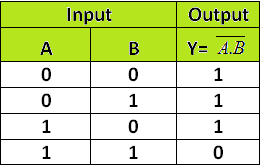
\includegraphics[width=\linewidth, height=40mm]{Unknown-5.jpeg}
			\end{minipage}
		&
		%\begin{minipage}{t}{5cm}
		\begin{itemize}
			\item Easy to contribute to your open source projects
			\item Documentation
			\item Showcase your work \ldots
			\item Track changes in your code across versions
			\item Integration options
		\end{itemize}
				%\end{minipage}
				&
				%\begin{minipage}{5cm}
				\begin{itemize}
					\item Continuous integration leads to problems
					\item Not an easy tool for beginners 
					\item Working with larger files can be tricky
				\end{itemize}
			%\end{minipage}
			\\
			\hline
		\end{tabular}
	\caption{Github Analysis}\label{tbl:mygitHub}
			
		
	\end{table}
\end{document}